بازی بی‌نهایت تکرارشونده زیر را درنظر بگیرید به طوری که در آن ضریب
$\delta$
به صورت 
$\delta \in (0, 1)$
باشد.

\begin{center}
    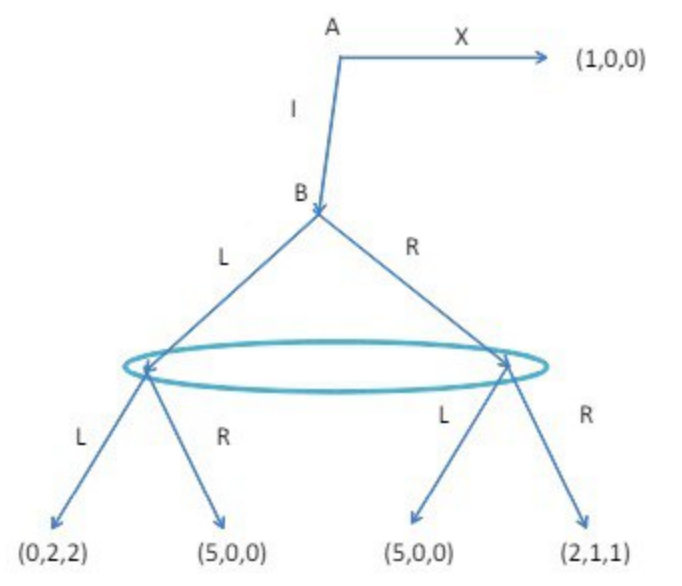
\includegraphics[width=0.5\linewidth]{pics/image1}
\end{center}

برای هر کدام از پروفایل‌های استراتژی زیر، محدوده‌ای از
$\delta$
را پیدا کنید که در آن پروفایل استراتژی یک تعادل نش متعالی زیربازی باشد.

\vspace*{5pt}
\textbf{الف)}
اگر
$(I, L, R)$
در تمام روزهای قبلی بازی شده باشد، بازی
$(I, L, R)$
انجام می‌شود و در غیر این صورت
$(X, L, L)$
بازی می‌شود.

\vspace*{5pt}
\textbf{ب)}
در "یکشنبه‌ها"، یعنی در 
$t \in \{0,7,14, \ldots\}$،
$(X, L, L)$
بازی می‌شود؛ در روزهای دیگر، اگر
$(I, L, R)$
در تمام روزهای قبلی بازی شده باشد،
$(I, L, R)$
بازی می‌شود و در غیر این صورت
$(X, L, L)$
بازی می‌شود.

\vspace*{5pt}
\textbf{ج)}
در "یکشنبه‌ها"،
$(X, L, L)$
بازی می‌شود؛ در روزهای دیگر، اگر
$(I, R, R)$
در تمام روزهای قبلی بازی شده باشد،
$(I, R, R)$
بازی می‌شود و در غیر این صورت
$(X, L, L)$
بازی می‌شود.